\subsection{Aufbau}
In diesem Experiment zum Photoeffekt sieht der Versuchsaufbau wie in Abbildung \ref{fig:Aufbau} aus. Gemessen wird der Photostrom am Ampèremeter in Abhängigkeit von der angelegten Gegenspannung. Das \glqq zylindrische Gehäuse\grqq\ beinhaltet die Photozelle. Eine Photozelle besteht aus einem evakuierten Glaskolben und zwei Elektroden. Eine davon ist die Photokathode. Sie besteht aus einer aufgedampften Metall- oder Legierungsschicht. Diese Schicht wird vom Licht bestrahlt. Die andere Elektrode, die Auffangelektrode, ist ein Drahtring, der wenige Millimeter neben der Kathodenoberfläche verläuft.
\begin{figure}[h!]
	\centering
	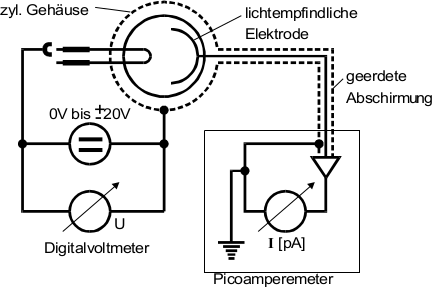
\includegraphics[width = 0.5\textwidth]{Aufbau.png}
	\caption{Verwendeter Versuchsaufbau \cite{\V}}
	\label{fig:Aufbau}
\end{figure}
Um Licht verschiedener Wellenlängen, also verschiedener Frequenzen, messen zu können wird zusätzlich noch eine Kombination aus Linsen (siehe Abbildung \ref{fig:Linsen}) benötigt. Das Prisma sorgt dafür, dass das Licht der \ce{Hg}-Lampe in seine Spektrallinien aufgeteilt wird. Die Linsen werden dann so verschoben, dass die Linien möglichst scharf erkennbar sind. Mit dem Schwenkarm kann das Schutzgehäuse, indem die Photozelle sitzt, so nach links und rechts verschoben werden, dass die gewünschte Spektrallinie durch den Eintrittspalt fällt.
\begin{figure}[h!]
	\centering
	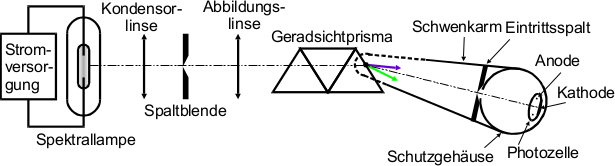
\includegraphics[width = 0.7\textwidth]{OptischerAufbau.png}
	\caption{Optischer Aufbau, der benötigt wird um mit einer Spektrallampe Licht verschiedener Frequenzen messen zu können \cite{\V}}
	\label{fig:Linsen}
\end{figure}

\subsection{Mögliche Schwierigkeiten dieses Aufbaus}
Die Messung kann durch verschiedene Faktoren vom erwarteten Ergebnis abweichen.
\begin{enumerate}
	\item Die Photoelektronen sind nicht monoenergetisch, da die Elektronen schon vorher im gebundenen Zustand verschiedene Energien hatten (Die Energieverteilung wird durch die Fermi-Dirac-Statistik beschrieben, wobei $0\leq E\leq\zeta$ (Fermi-Energie) gilt.). Das sorgt dafür, dass der Photostrom bei der Grenzspannung nicht sofort und schlagartig verschwindet, sondern absinkt und erst bei einer Spannung $U<U_\text{g}$ nicht mehr vorhanden ist. (siehe Abbildung \ref{fig:UI})
	\item Die Austrittsarbeit des Anodenmaterials $A_\text{A}$ ist sehr groß, insbesondere größer, als die Austrittsarbeit des Kathodenmaterials $A_\text{K}$. Es kann dann passieren, dass die Elektronen aus der Kathode austreten können, da $h\nu>A_\text{K}$, aber kein Photostrom gemessen werden kann, weil die Energie der Elektronen kleiner ist, als die Fermi-Energie des Anodenmaterials. Um dennoch einen Photostrom messen zu können, muss die angelegte Spannung beschleunigend wirken.
\end{enumerate}
\begin{figure}[h!]
	\centering
	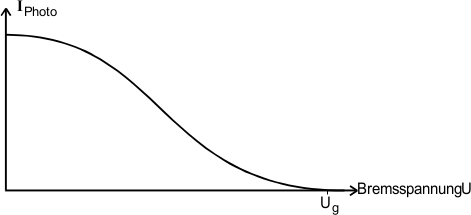
\includegraphics[width = 0.6\textwidth]{IU.png}
	\caption{Photostrom in Abhängigkeit von der Bremsspannung bei einer mit monochromatischem Licht bestrahlten Photozelle \cite{V500}}
	\label{fig:UI}
\end{figure}
Werden die beschriebenen Schwierigkeiten beachtet und bestimmte Annahmen gemacht, gilt der Zusammenhang
\begin{align}
	I \propto U^2
\end{align}
zwischen dem Photostrom $I$ und der angelegten Spannung $U$.